\documentclass[11pt]{article}
\usepackage{hyperref}
\usepackage{amsthm}
\usepackage{amsmath}
\usepackage{amsfonts}
\usepackage{tikz}
\usepackage{ wasysym }

\newtheorem{example}{Example}


\author{}
\title{}

\begin{document}
%\maketitle
{\Large
%Change Document name to: Graded Homework 1\_Jacob\_Nicholas
\noindent NAME:  Nicholas Jacob\\ 
STUDENT ID: \# 113578513\\
GRADED HOMEWORK NUMBER: 3\\
COURSE: CS/DSA 4513 DATABASE MANAGEMENT\\ 
SECTION: ONLINE\\SEMESTER: FALL 2023\\
INSTRUCTOR:  DR. LE GRUENWALD\\
 SCORE:}

\newpage
\begin{enumerate} \item Screenshots
\begin{enumerate}
\item 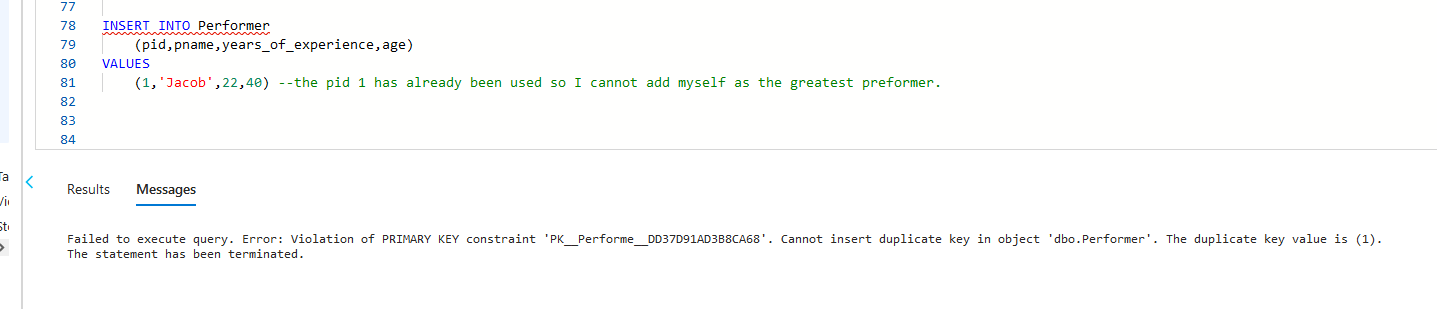
\includegraphics[width = \textwidth]{primaryKeyViolation.png} 
\item 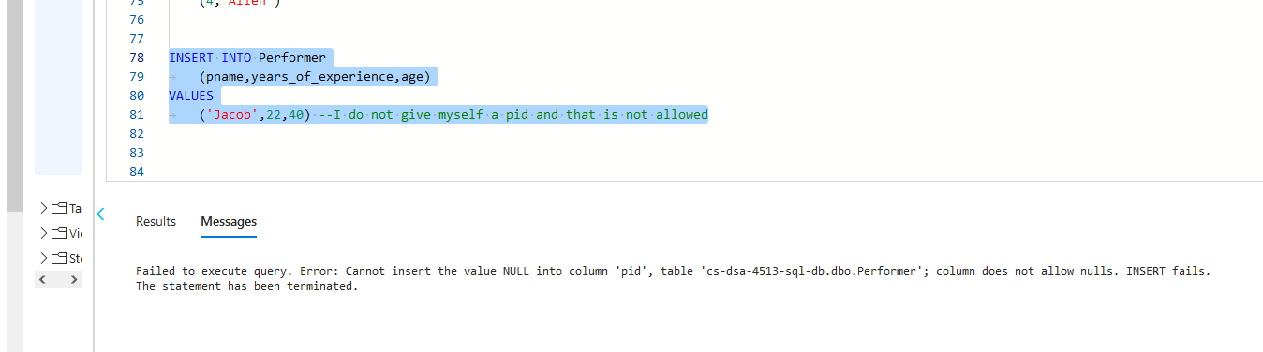
\includegraphics[width = \textwidth]{noKeyViolation.png} 
\item 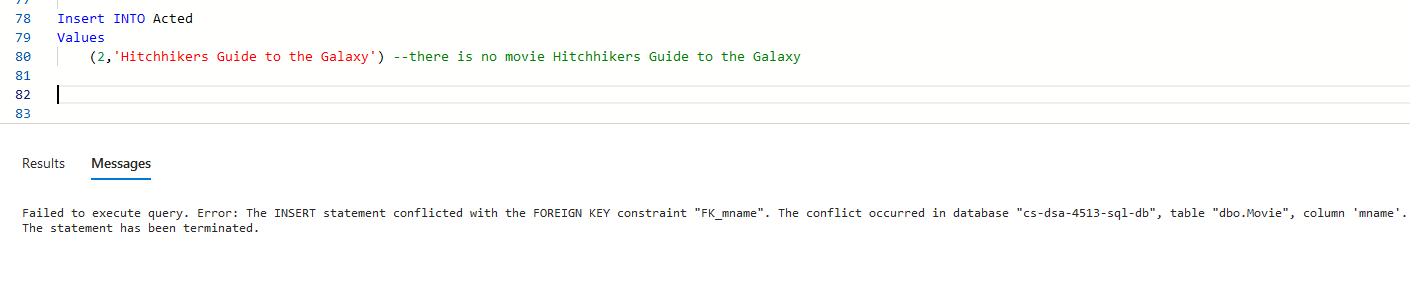
\includegraphics[width = \textwidth]{fKeyViolation.png} 
 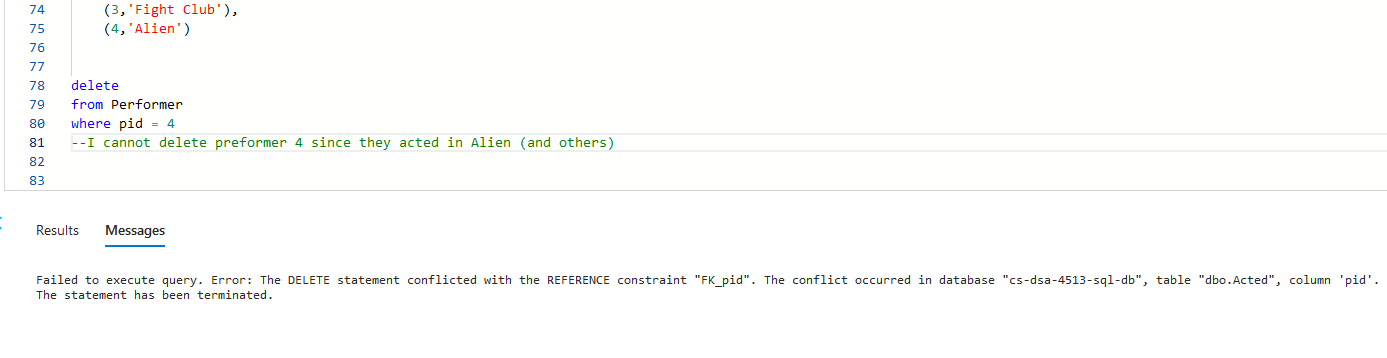
\includegraphics[width = \textwidth]{fKeyViolationDelete.png} 
 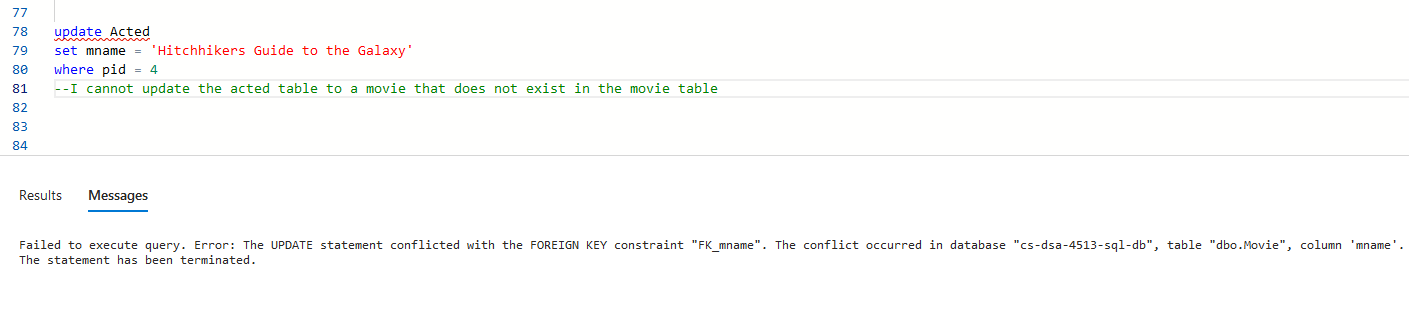
\includegraphics[width = \textwidth]{fKeyViolationUpdate.png} 
\item 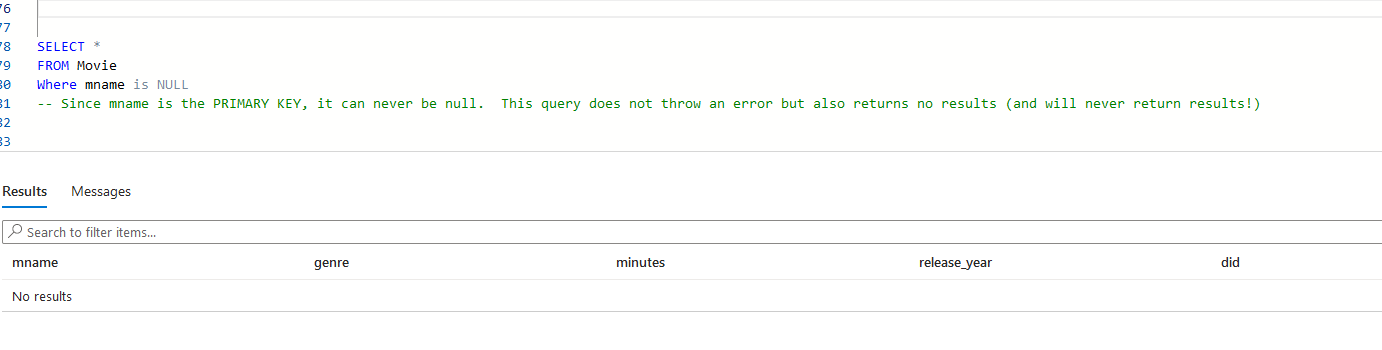
\includegraphics[width = \textwidth]{select.png} 
\end{enumerate}
\item I choose to index the Movie table on genre attribute.  We had three queries that used genre so it was not a terrible option for indexing.  It was a secondary index since mname was the primary index (and primary key). 

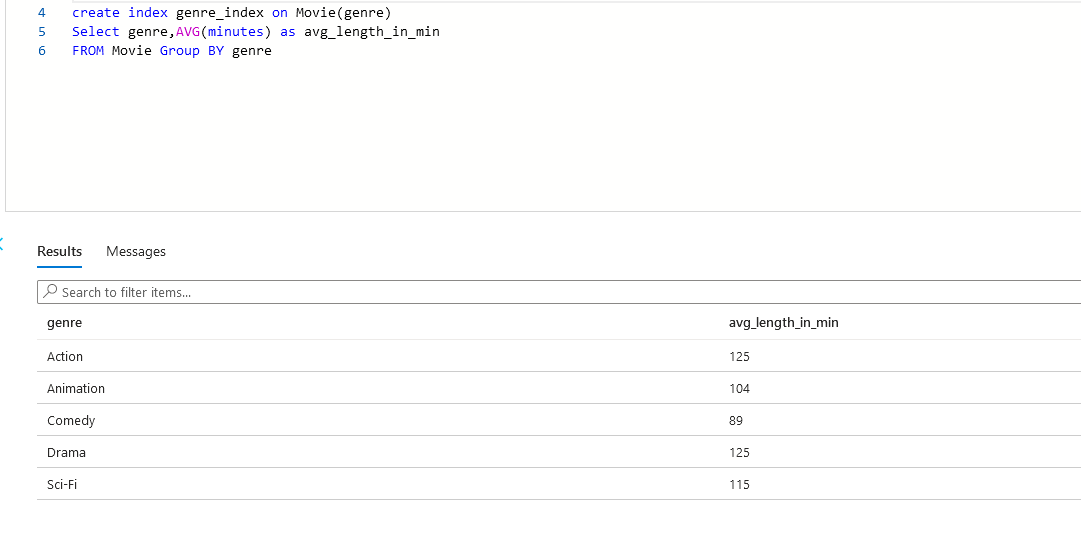
\includegraphics[width=\textwidth]{selectWithIndex.png}
\end{enumerate}






\end{document}